\documentclass[12pt]{report}

%IMPORTS
\usepackage[catalan]{babel}
\usepackage[utf8]{inputenc}
\usepackage{graphicx}
\usepackage{wrapfig}
\usepackage{amsmath}
\usepackage{amssymb}
\usepackage{ragged2e} 
\usepackage{subfig}
\usepackage{caption}
\usepackage{subcaption}
\usepackage[usenames]{color}
\usepackage{xcolor}
\usepackage{float}
\usepackage{chngcntr}
\usepackage{ragged2e}
\usepackage{multirow}
\usepackage{vmargin}
\usepackage{hyperref}

\title{Pràctica 1: Fractals generats pel mètode de Newton}
\author{Gerard Lahuerta Martín}
\date{ 30 d'abril del 2021}

\setpapersize{A4}
\setmargins{3cm}       % margen izquierdo
{2.6cm}                % margen superior
{16.5cm}               % anchura del texto
{23.7cm}               % altura del texto
{10pt}                 % altura de los encabezados
{0cm}                  % espacio entre el texto y los encabezados
{0pt}                  % altura del pie de página
{1cm}                  % espacio entre el texto y el pie de página
\renewcommand{\baselinestretch}{1.5}

\begin{document}
\justifying
\maketitle


\newpage
\setcounter{page}{2}
\pagestyle{plain}
\tableofcontents
\cleardoublepage
\addcontentsline{}{chapter}{}


%%%%%%%%%%%%%%%%%%%%%%%%%%%%%%%%%%%%%%%%%%%%%%%%%%%%%%%%%%%%%%%%%%%%
\newpage
\chapter{Introducció al treball}
\justifying
\section{Motivació del treball}
Aquest treball ha estat motivat per l'empresa de disseny al precisar un conjunt de rutines que generin fractals mitjançant el mètode de Newton. Per tal de donar alguns casos de referència també s'ha procedit a programar una utilitat mitjançant el programa gnuplot i la línia d'ordres d'Unix.


%%%%%%%%%%%%%%%%%%%%%%%%%%%%%%%%%%%%%%%%%%%%%%%%%%%%%%%%%%%%%%%%%%%%
\section{Metodologia}
\subsection{Explicació de la metodologia}
La metodologia utilitzada alhora de programar el codi es la següent:
\begin{enumerate}
    \item Llenguatge de programació ràpid i eficient
    \newline
    Utilitzem el llenguatge C gràcies a la rapidesa en els càlculs i l'alta eficiència.
    \item Fàcil d'executar
    \newline
    La programació ha estat orientada a la fàcil utilització d'aquest per tal de ser intuïtiva, a més, s'afegeix el manual d'ús del software per les consultes necessàries.
    \item Fàcil modificació
    \newline
    El programa està forçament comentat i enfocat per a ser fàcilment intuïtiu per si calgués alguna modificació a posterior i, així, facilitar la tasca.
\end{enumerate}


%%%%%%%%%%%%%%%%%%%%%%%%%%%%%%%%%%%%%%%%%%%%%%%%%%%%%%%%%%%%%%%%%%%%
\subsection{Comentaris}
El disseny de les rutines ha estat pensat i implementat per a evitar els càlculs i interaccions innecessàries. També, s'ha evitat la creació de rutines i variables redundants per a obtenir la millor optimització possible.
\newline 
Tal com hem comentat anteriorment, per tal d'evitar confusions i ajudar a l'enteniment de les accions del programa s'han implementat línies de codi comentat, aquestes expliquen els conceptes més ambigus del programa i estan localitzades al costat de cada línia on s'ha cregut necessària una explicació.

%%%%%%%%%%%%%%%%%%%%%%%%%%%%%%%%%%%%%%%%%%%%%%%%%%%%%%%%%%%%%%%%%%%%
\subsection{Informació adicional d'interés}
La biblioteca ha estat programada amb l'editor d'ús públic Notepad++, encara que pot ser modificat en altres editors com podrien ser l'editor de notes o d'altres més complexos com VisualStudio.
\newline
Durant la programació de les rutines s'ha ideat un programa per testejar el correcte funcionament de la biblioteca i així en cas de possibles errors poder comprovar el correcte funcionament d'aquesta.
\newline
L'ús d'aquest test que està anomenat com
\textit{test$\_$avalp} 
és fàcilment executable i és explicat més a fons a la \subsectionautorefname{ 2.1.4 test$\_$avalp i el funcionament correcte de la biblioteca}


%%%%%%%%%%%%%%%%%%%%%%%%%%%%%%%%%%%%%%%%%%%%%%%%%%%%%%%%%%%%%%%%%%%%
\chapter{Explicació de la biblioteca}
En aquest capítol parlarem a fons sobre l'estructura, els materials que implementa, el funcionament, les estratègies utilitzades i el correcte ús i execució del programa.


%%%%%%%%%%%%%%%%%%%%%%%%%%%%%%%%%%%%%%%%%%%%%%%%%%%%%%%%%%%%%%%%%%%%
\section{Funcionament}
La biblioteca està pensada per a ser implementada en els entorns d'execució de l'empresa de disseny i no per a substituir els mateixos.
\newline
Els mètodes que s'inclouen en la biblioteca (dels quals parlem a continuació) poden ser utilitzats independentment i no precisa cap altra eina externa més enllà de la llibreria \textit{math.h} del conjunt de llibreries del llenguatge C.
\subsection{Càlcul dels fractals}
El mètode matemàtic que hem utilitzat per a saber de manera aproximada les òrbites dels punts que generen els fractals és el mètode de Newton de manera iterativa.
\newline
A partir d'un punt $z_0=a+bi\in\mathbb{C}$, amb $a,b\in\Re$ (coordenades de l'eix x, y; coordenades del píxel de la pantalla), calculem la seva òrbita després de $K\in\Re$ iteracions de la següent manera:
\newline
$z_1=z_0-\frac{p(z_0)}{p'(z_0)} \longrightarrow z_2=z_1-\frac{p(z_1)}{p'(z_1)} \longrightarrow z_3=z_2-\frac{p(z_2)}{p'(z_2)} \longrightarrow \cdots \longrightarrow z_k=z_{k-1}-\frac{p(z_{k-1})}{p'(z_{k-1})}$ $$z_j=z_{j-1}-\frac{p(z_{j-1})}{p'(z_{j-1})}, \forall j \in \{1, \cdots, K\}$$
Essent $p(z)\in\mathbb{C}_t[Z]$ expressat de forma factoritzada; on $z\in\mathbb{C}$, $t\in\mathbb{N}$ el nombre d'arrels.


%%%%%%%%%%%%%%%%%%%%%%%%%%%%%%%%%%%%%%%%%%%%%%%%%%%%%%%%%%%%%%%%%%%%
\subsection{Organització}
\justifying
La biblioteca \textit{nwtfr.h} ha estat organitzada de manera que totes les funcions han estat programades en un sol fitxer per així facilitar la implementació de la biblioteca en el software de l'empresa.
\newline
Per a fer els càlculs mitjançant el mètode de Newton hem dividit el treball en tres funcions que depenen entre elles: la funció \textit{avalp} (avalua el polinomi), la funció \textit{avaldp} (avalua la derivada del polinomi) i la funció \textit{cnvnwt} (calcula l'arrel del polinomi a la que s'aproxima $z_0$ mitjançant el mètode de newton). Expliquem aquestes tres funcions amb més profunditat en els següents subapartats.
\newline
La dependència de les funcions \textit{avalp}, \textit{avaldp} i cnvnwt és piramidal, de manera que les funcions deleguin càlculs en altres funcions per a optimitzar i organitzar millor el codi.
\newline
La funció per a dur a terme tots els càlculs del fractal és l'anomenada cnvnwt i que crida a les funcions \textit{avalp} i \textit{avaldp} que analitzaran el polinomi que genera el fractal i la seva derivada.

\begin{center}
    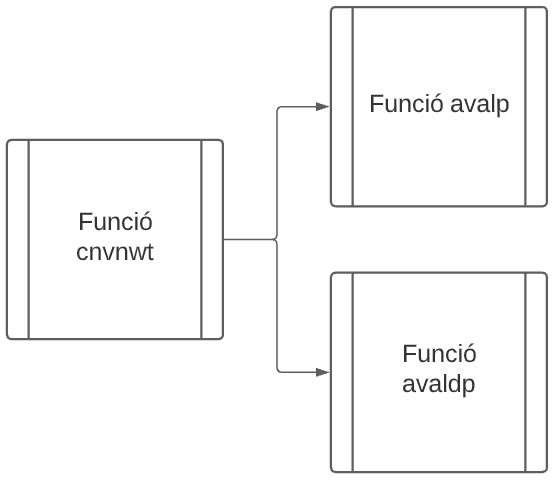
\includegraphics[width=0.8\textwidth]{diarama_dependencies.PNG}
    \newline
Diagrama de flux de les dependències entre les funcions de la biblioteca
\label{fig:UML_funcionsgeneral}
\end{center}



%%%%%%%%%%%%%%%%%%%%%%%%%%%%%%%%%%%%%%%%%%%%%%%%%%%%%%%%%%%%%%%%%%%%
\subsection{Biblioteca nwtfr.c}
Expliquem a continuació el funcionament i composició dels mètodes i com compilar-los.

%%%%%%%%%%%%%%%%%%%%%%%%%%%%%%%%%%%%%%%%%%%%%%%%%%%%%%%%%%%%%%%%%%%%
\subsubsection{Mètode avalp}
El mètode avalp és l'encarregat de calcular el valor $p(z_0)$ a partir dels valors $a,b\in\Re/z_0=a+bi$ la llavor, $\{w_1, \cdots, w_n \hspace{0.5em} / \hspace{0.5em} w_q=\alpha+\beta i \hspace{0.5em}\forall q\in\{1, \cdots n\}, \hspace{0.25em}\alpha,\beta\in\Re\}$ les arrels de $p(z)$ essent $n\in\mathbb{N}$ el nombre d'arrels del polinomi.
\newline
Per fer l'avaluació, els arguments que es passen al mètode de manera consecutiva són els següents:
\begin{itemize}
    \item [$\bullet$] Variables double \textit{x} i \textit{y}: són els valors de $z\in\mathbb{C}$ que s'introdueixen per a calcular el valor de $p(z)$; és a dir, $z=x+y\cdot i$ amb $x,y\in\Re$.
    \item [$\bullet$] Apuntadors de tipus double \textit{px} i \textit{py}: són les adreces de memòria on es guardaran el valor de $p(z)$; és a dir, $p(z)=px+py\cdot i$.
    \item [$\bullet$] Variable integuer \textit{n}: és el nombre d'arrels del polinomi $p(z)$; indica, per tant, la llargada de les llistes que contenen els valors de les arrels del polinomi.
    \item [$\bullet$] Llistes del tipus double \textit{u} i \textit{v}: són les llistes que contenen totes les arrels del polinomi $p(z)$ de manera que:
    \begin{equation*}
        p(z)=\prod_{\substack{q=1}}^n(z-w_q)
    \end{equation*}
    Amb $w_q=\alpha_q+\beta_q i \hspace{0.5em}\forall q\in\{1, \cdots n\}, \hspace{0.5em}\alpha_q,\beta_q\in\Re$ de manera que els valors de $\alpha_q$ és guardada a la posició $q$-èssima de la llista $\textit{u}$ i $\beta_q$ és guardada a la posició $q$-èssima de la llista $v$.
\end{itemize}

\begin{center}
    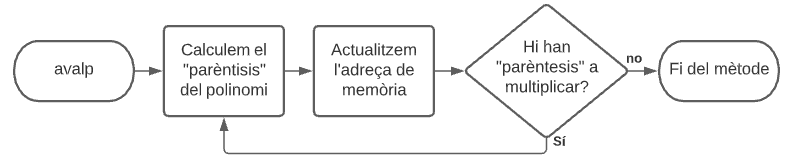
\includegraphics[width=1\textwidth]{UML_avalp.PNG}
    \newline
Diagrama de flux del mètode \textit{avalp}
\label{fig:UML_avalp}
\end{center}


%%%%%%%%%%%%%%%%%%%%%%%%%%%%%%%%%%%%%%%%%%%%%%%%%%%%%%%%%%%%%%%%%%%%
\subsubsection{Mètode avaldp}
El mètode \textit{avaldp} és l'encarregat de calcular el valor $p'(z_0)$ a partir dels mateixos valors que l'hi són introduïts a la funció \textit{avalp} pel que els donarem per definits (tornar al punt 2.1.3 Mètode avalp per veure els valors utilitzats).
\newline
Per fer l'avaluació, els arguments que es passen són similars al del mètode \textit{avalp}, per tant de forma consecutiva són els següents:
\begin{itemize}
    \item [$\bullet$] Variables double \textit{x} i \textit{y}: són els valors de $z\in\mathbb{C}$ que s'introdueixen per a calcular el valor de $p'(z)$; és a dir, $z=x+y\cdot i$ amb $x,y\in\Re$.
    \item [$\bullet$] Apuntadors de tipus double \textit{dpx} i \textit{dpy}: són les adreces de memòria on és guardaran el valor de $p'(z)$; és a dir, $p(z)=dpx+dpy\cdot i$.
    \item [$\bullet$] Variable integuer \textit{n}: és el nombre d'arrels del polinomi $p(z)$; indica, per tant, la llargada de les llistes que contenen els valors de les arrels del polinomi.
    \item [$\bullet$] Llistes del tipus double \textit{u} i \textit{v}: són les llistes que contenen totes les arrels del polinomi $p(z)$ de manera que:

        \[p'(z)= \sum_{\begin{subarray} \text{k}=0\end{subarray}}^{n-1} \prod_{\substack{q=0\\q\ne k}}^{n-1}(z-w_q) \]

    Amb $w_q$ definida de la mateixa manera que a la funció \textit{avalp}.
\end{itemize}

\begin{center}
    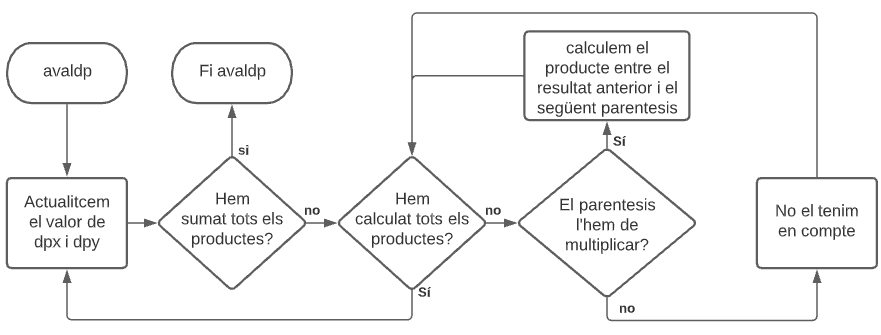
\includegraphics[width=1\textwidth]{UML_avaldp.PNG}
     \newline
Diagrama de flux del mètode \textit{avaldp}
\label{fig:UML_avalp}
\end{center}

%%%%%%%%%%%%%%%%%%%%%%%%%%%%%%%%%%%%%%%%%%%%%%%%%%%%%%%%%%%%%%%%%%%%
\subsubsection{Mètode cnvnwt}
El mètode cnvnwt és l'encarregat de calcular el valor de la posició de la llista que contè l'arrel del polinomi $p(z)$ que la llavor $z_0=x+y\cdot i$ s'aproxima amb una certa tolerancia, $tolcnv$, en un màxim d'iteracions establertes, $maxit$. Per això utilitza els mètodes abans explicats de \textit{avalp} i \textit{avaldp}. Els arguments necesaris de \textit{cnvnwt}, consecutivament, són:
\begin{itemize}
    \item [$\bullet$] Variables double \textit{x} i \textit{y}: són els valors de $z_0=x+y\cdot i\in\mathbb{C}$ que s'introdueixen per a calcular la seva òrbita, amb $x,y\in\Re$.
\item [$\bullet$] Variable double \textit{tolcnv}: és la distància mínima que ha d'estar un punt de l'òrbita de $z_0$ per ser considerada com a valor zero i retornar el valor de la posició d'aquesta arrel.
\item [$\bullet$] Variable integuer \textit{maxit}: és el valor màxim d'iteracions que durà a terme el mètode cnvnwt per tal de calcular a quina arrel s'aproxima l'òrbita de $z_0$.
\item [$\bullet$] Variable integuer \textit{n}: és el nombre d'arrels del polinomi $p(z)$; indica, per tant, la llargada de les llistes que contenen els valors de les arrels del polinomi.
\item [$\bullet$] Llistes del tipus double \textit{u} i \textit{v}: són les llistes que contenen totes les arrels del polinomi $p(z)$ que s'utilitzaran per a calcular la distància entre els punts de l'òrbita i les arrels de $p(z)$, calcular el valor de $p(z)$ amb el mètode \textit{avalp} i calcular i $p'(z)$ amb \textit{avaldp}.
\end{itemize}
Comentar també que en cas que algun $z_0$ no s'aproximés a cap arrel, aquesta funció retornarà el valor $-1$ per a indicar aquest fenomen.

\begin{center}
    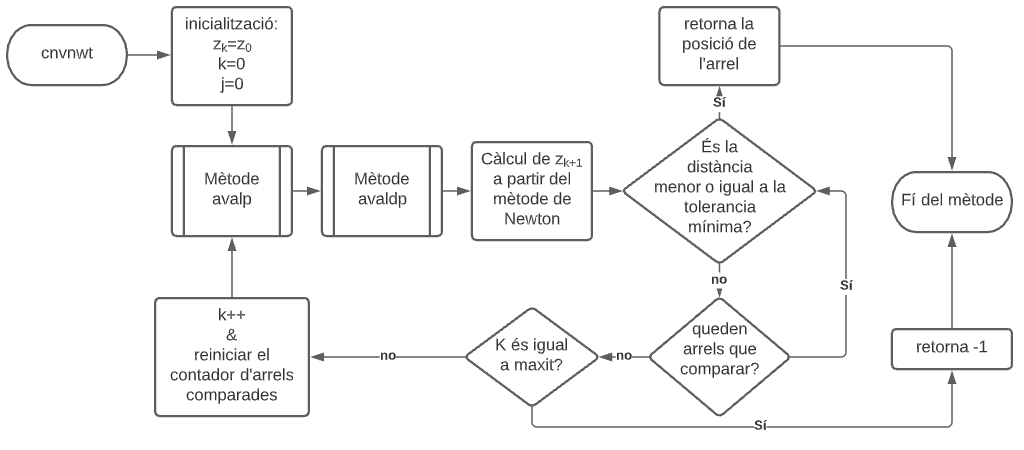
\includegraphics[width=1\textwidth]{UML_cnvnwt.PNG}
     \newline
Diagrama de flux del mètode \textit{cnvnwt}
\label{fig:UML_avalp}
\end{center}



%%%%%%%%%%%%%%%%%%%%%%%%%%%%%%%%%%%%%%%%%%%%%%%%%%%%%%%%%%%%%%%%%%%%
\subsubsection{Compilació de la biblioteca i document Makefile}
Per a poder organitzar de millor manera la compilació de la biblioteca, així com la seva implementació al programa \textit{dibfr.c} (que és el programa encarregat de fer els càlculs necessaris per a representar els fractals i que en la següent secció expliquem en profunditat); hem creat un arxiu que s'encarrega de la seva compilació.
Aquest arxiu porta el nom \textit{Makefile} seguit d'una barra baixa i el nom del sistema operatiu pel qual ha estat pensat.
\newline
A l'empresa només l'interessa utilitzar el fitxer \textit{Makefile$\_$Unix.txt}, però igualment s'ha volgut crear una còpia modificada del fitxer per si es precisa fer modificacions del programa amb un software o plataforma de Windows. Si és aquest el cas, utilitzar l'arxiu \textit{Makefile$\_$Windows.txt}.
\newline
L'execució dels arxius Makefile, encarregats de la compilació de l'executable encarregat de fer el fitxer amb la informació per després dibuixar els fractals amb el \textit{gnuplot}, és senzilla.
\begin{itemize}
\item [$\circ$] \textbf{Si es tracta del sistema Operatiu Unix}, en la consola/terminal de l'ordinador executar la comanda \textit{make -f Makefile$\_$Unix.txt} per crear l'executable \textit{dibfr}.
\newline
Anàlogament, executar la comanda \textit{clean -f Makefile$\_$Unix.txt} per netejar \textit{d'arxius objecte} innecessaris el directori de treball o \textit{realclean -f Makefile$\_$Unix.txt} per esborrar tot el treball fet per l'arxiu Makefile.
\item [$\circ$] \textbf{Si es tracta del sistema Operatiu Windows}, en la consola/terminal de \textit{mingw-w64} executar la comanda \textit{mingw32-make -f Makefile$\_$Windows.txt} per crear l'executable \textit{dibfr.exe}.
\newline
Anàlogament, executar la comanda \textit{minw32-make clean -f Makefile$\_$Windows.txt} per netejar d'arxius objecte innecessaris el directori de treball o \textit{minw32-make realclean -f Makefile$\_$Unix.txt} per esborrar tot el treball fet per l'arxiu Makefile.
\end{itemize}
Esmentar que sobre l'arxiu del codi del programa \textit{dibfr.c} es comentarà més endavant a la Secció 2.1.5 Programa dibfr.c i executable dibfr, on es parlarà més a fons sobre el codi que s'utilitza, la implementació de la biblioteca en el codi i el seu ús en \textit{gnuplot} en la representació de fractals.
\newpage
%%%%%%%%%%%%%%%%%%%%%%%%%%%%%%%%%%%%%%%%%%%%%%%%%%%%%%%%%%%%%%%%%%%%
\subsection{test$\_$avalp i el funcionament correcte de la biblioteca}
Expliquem a continuació el programa \textit{test$\_$avalp} i la correcta implementació de la biblioteca en els codis de programació de l'empresa així com en el mateix codi.
\subsubsection{Implementació i correcta utilització de la biblioteca \textit{nwtfr.h}}
Per a implementar a biblioteca \textit{nwtfr.h} en qualsevol codi en C cal a l'inici del codi escriure la comanda següent:
$$\textbf{\textit{\#include "nwtfr.h"}}$$
Una vegada escrita la comanda el programa implementarà els mètodes de l'extensió al codi.
\newline
Si no s'utilitza l'arxiu Makefile, explicat en el passat apartat, es pot compilar els arxius que continguin aquesta biblioteca amb la comanda següent al terminal/consola:
$$\textbf{\textit{gcc -o nom\_del\_executable -Wall nom\_del\_programa.c nwtfr.c}}$$
%%%%%%%%%%%%%%%%%%%%%%%%%%%%%%%%%%%%%%%%%%%%%%%%%%%%%%%%%%%%%%%%%%%%

\subsubsection{Programa i executable \textit{test$\_$avalp}}
Per tal d'assegurar el funcionament correcte de la biblioteca hem posat a disposició de l'empresa el codi \textit{test\_avalp} que té com a objectiu assegurar que els mètodes que actualment conté la biblioteca funcionin de manera correcta.
\newline
El programa \textit{test\_avalp} és molt senzill, únicament crida les tres funcions que conté \textit{nwtfr.h} per fer uns càlculs de prova i eventualment mostrar-los per pantalla.
\newline
Per obtenir l'executable utilitzem la comanda abans explicada,
$$\textbf{\textit{gcc -o test\_avalp -Wall test\_avalp.c nwtfr.c}}$$
Una vegada obtingut l'executable \textit{test\_avalp} (o \textit{test\_avalp.exe} si es tracta d'un dispositiu Windows) cal executar-lo per consola.
\begin{center}
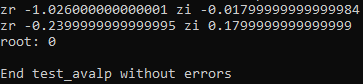
\includegraphics[width=1\textwidth]{test_avalp.PNG}
\newline
Missatge de sortida en executar \textit{test\_avalp} si la biblioteca funciona correctament
\label{fig:UML_avalp}
\end{center}

%%%%%%%%%%%%%%%%%%%%%%%%%%%%%%%%%%%%%%%%%%%%%%%%%%%%%%%%%%%%%%%%%%%%
\subsection{Programa dibfr.c i executable dibfr}
En aquesta secció explicarem el funcionament del programa \textit{dibfr}, el seu funcionament intern i les seves dependències.
\newline
També comentarem com utilitzar la informació obtinguda per a representar els fractals per pantalla mitjançant el programa d'accés lliure i gratuït de gnuplot.


%%%%%%%%%%%%%%%%%%%%%%%%%%%%%%%%%%%%%%%%%%%%%%%%%%%%%%%%%%%%%%%%%%%%
\subsubsection{Dependencies i necessitats del programa}
El programa \textit{dibfr} depèn íntegrament de la biblioteca \textit{nwtfr.h}. Concretament utilitza la funció \textit{cnvnwt} que calcula l'arrel a la qual l'òrbita d'un $z_0$ l'anul·la.
\newline
El programa per ser executat requereix certs arguments que s'han d'acompanyar a l'hora d'executar; és a dir, s'ha d'introduir al terminal de l'Unix la comanda:
$$./dibfr \hspace{0.5em} narr \hspace{0.5em} xmn \hspace{0.5em} xmx \hspace{0.5em} nx\hspace{0.5em}  ymn \hspace{0.5em} ymx \hspace{0.5em} ny \hspace{0.5em} tolcnv \hspace{0.5em} maxit$$
(En cas de ser utilitzada en un terminal de Windows, eliminar el $./$ a l'inici de la comanda)
\newline
Aquestes variables que hem anomenat a posteriori de l'executable són:
\begin{itemize}
    \item [$\blacktriangleright$] \textbf{variable \textit{narr}:} integuer que determina el nombre d'arrels de $p(z)$.
    \item [$\blacktriangleright$] \textbf{variable \textit{xmn}:} valor mínim que pot tenir la part real de la llavor $z_0$.
    \item [$\blacktriangleright$] \textbf{variable \textit{xmx}:} valor màxim que pot tenir la part real de la llavor $z_0$.
    \item [$\blacktriangleright$] \textbf{variable \textit{nx}:} nombre d'intervals a dividir el segment $\overline{xmn \hspace{0.5em} xmx}$.
    \item [$\blacktriangleright$] \textbf{variable \textit{ymn}:} valor mínim que pot tenir la part imaginària de la llavor $z_0$.
    \item [$\blacktriangleright$] \textbf{variable \textit{ymx}:} valor màxim que pot tenir la part imaginària de la llavor $z_0$.
    \item [$\blacktriangleright$] \textbf{variable \textit{ny}:} nombre d'intervals a dividir el segment $\overline{ymn \hspace{0.5em} ymx}$.
    \item [$\blacktriangleright$] \textbf{variable \textit{tolcnv}:} tolerància màxima per aplicar al càlcul de la funció \textit{cnvnwt}
    \item [$\blacktriangleright$] \textbf{variable \textit{maxit}:} nombre màxim d'iteracions que pot fer la funció \textit{cnvnwt}.
\end{itemize}
Aquesta comanda executarà el programa \textit{dibfr} i mostrarà per pantalla tota la informació que calcula.
\newline
\textit{Expliquem a la següent secció la informació que retorna, com utilitzar-la i el procés que segueix per a obtenir-la}.

%%%%%%%%%%%%%%%%%%%%%%%%%%%%%%%%%%%%%%%%%%%%%%%%%%%%%%%%%%%%%%%%%%%%
\subsubsection{Programa dibfr.c}
El programa \textit{dibfr.c}, com hem estat comentant, s'encarrega de fer els càlculs per a representar els fractals, i recordar també que, l'executable del programa es pot obtenir mitjançant el fitxer Makefile explicat en l'apartat anterior.
\newline
El funcionament de la mateixa (explicat al final de la secció) és senzilla, una vegada a llegit i guardat els arguments introduïts per pantalla (en la comanda abans explicada) el programa preguntarà tants cops com arrels ha decidit l'usuari que tingui els següents valors (que han de ser introduir seguits amb un espai entre ells):
\begin{itemize}
\item [$\diamond$] \textbf{Valor real de l'arrel}, aquest ha de ser un valor double
\item [$\diamond$] \textbf{Valor imaginari de l'arrel}, aquest ha de ser un valor double
\item [$\diamond$] \textbf{Color vermell en l'arrel}, aquest ha de ser $0$ o $1$, indica si l'arrel és vermella
\item [$\diamond$] \textbf{Color verd en l'arrel}, aquest ha de ser $0$ o $1$, indica si l'arrel és verda
\item [$\diamond$] \textbf{Color blau en l'arrel}, aquest ha de ser $0$ o $1$, indica si l'arrel és blava
\end{itemize}
\textit{En els valors dels colors, el valor 0 indicarà absència del mateix i 1 indicarà el color de l'arrel}
\newline
Un exemple d'introducció de la informació per pantalla una vegada executat \textit{dibfr}, introduïm l'arrel $z=1+0\cdot i$ i indiquem que serà de color vermell: $1 \hspace{0.5em} 0 \hspace{0.5em} 1 \hspace{0.5em} 0 \hspace{0.5em} 0$.
\newline
Els valors, respectivament, representen: el valor real de l'arrel $z$, el valor imaginari de l'arrel $z$, conté el color vermell, no conté el color verd i no conté el color blau.
\newline
Una vegada executat amb els arguments explicats i introduïts per consola els valors abans anomenats, el programa mostrarà per pantalla tota la informació, per la qual cosa es recomana a l'hora d'executar el programa per pantalla (just després dels arguments) col·locar una redirecció d'entrada a un fitxer per a contenir tota la informació allà i poder treballar de manera més còmoda amb el gnuplot (que explicarem a continuació d'aquesta secció).
\newline
Eventualment, cal mencionar que el funcionament de \textit{dibfr.c} es basa en obtenir la informació necessària per a poder fer les declaracions com a arguments (ja explicats), rebre la informació sobre els càlculs per pantalla (també explicada) i calcular els colors dels píxels de la pantalla tracta'n les coordenades X i Y de la pantalla com els components real i imaginari (respectivament) d'un nombre complex aplicant la funció \textit{cnvnwt} de la nostra biblioteca.
\begin{center}
    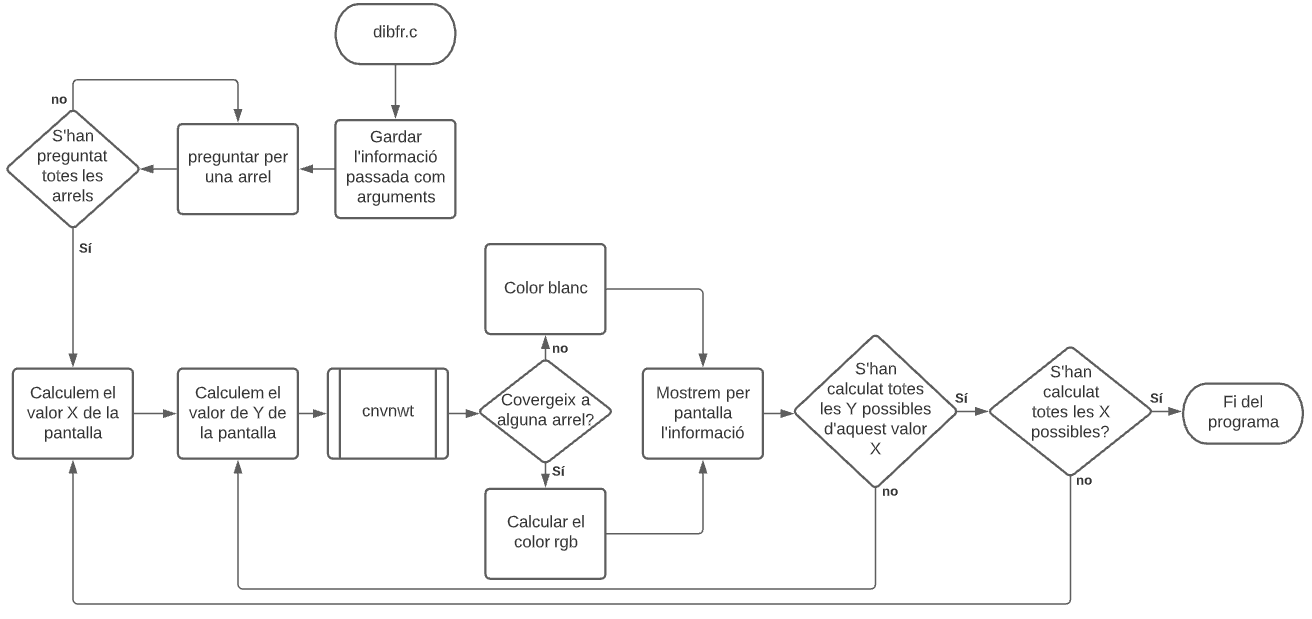
\includegraphics[width=1\textwidth]{UML_dibfr.PNG}
     \newline
Diagrama de flux de \textit{dibfr.c}
\label{fig:UML_dibfr}
\end{center}



%%%%%%%%%%%%%%%%%%%%%%%%%%%%%%%%%%%%%%%%%%%%%%%%%%%%%%%%%%%%%%%%%%%%
\subsubsection{Representació amb gnuplot}
En aquesta secció expliquem com representar per mitjà del software d'accés lliure \textit{gnuplot}.
\newline
Per a poder representar fractals a partir del \textit{gnuplot} ens situarem primerament en el directori on disposem de l'arxiu on hem recollit tota la informació obtinguda del programa \textit{dibfr}.
\newline
Una vegada en el directori, introduïm per pantalla les següents comandes:
\begin{itemize}
    \item [$>$] $\text{unset key}$
    \item [$>$] $\text{plot 'nom\_del\_fitcher\_amb\_l'informació.txt' using 1:2:3:4:5 with rgbimage}$
\end{itemize}
Per finalitzar, mostrarem a continuació una recopilació d'imatges de les representacions que hem obtingut seguint aquesta metodologia.
\newpage
\begin{center}
    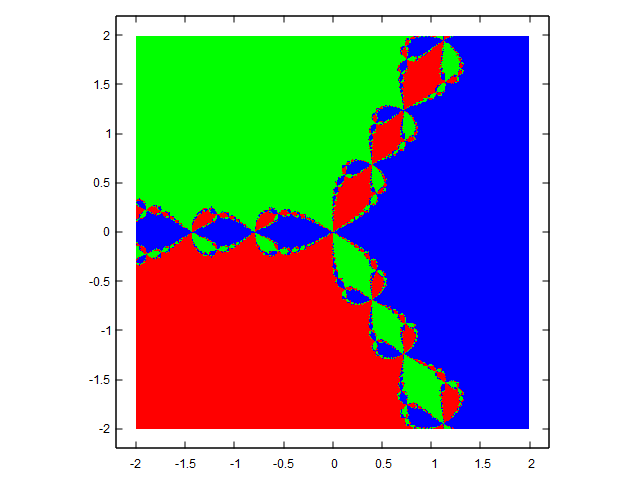
\includegraphics[width=0.6\textwidth]{z3-1.png}
    \newline
    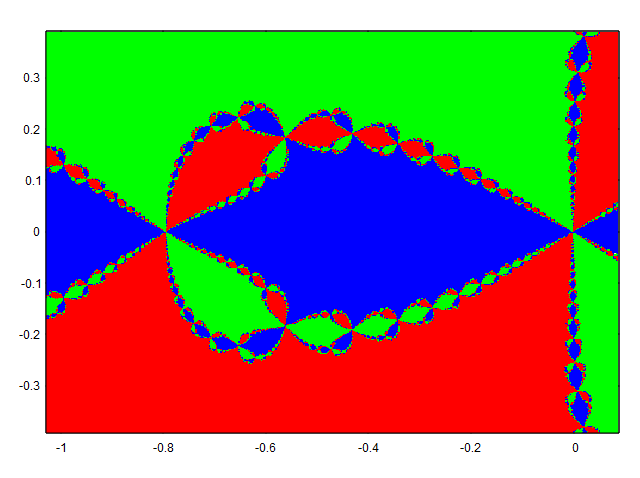
\includegraphics[width=0.6\textwidth]{z3-1_zoom.png}
    \newline
    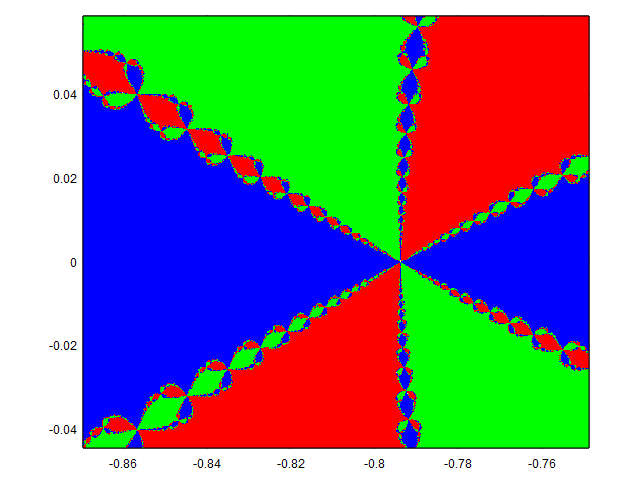
\includegraphics[width=0.6\textwidth]{z3-1_zoom2.png}
    \newline
Fractal dibuxat pel polinomi $p(z)=z^3-1$
\label{fig:z^3-1}
\end{center}

\newpage
\begin{center}
    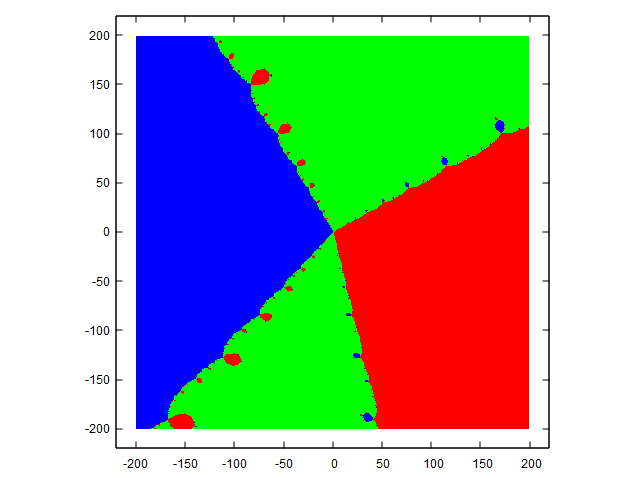
\includegraphics[width=0.6\textwidth]{mandel.png}
    \newline
    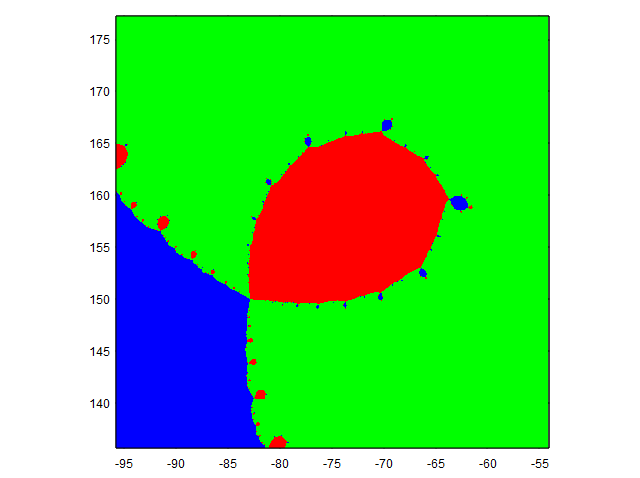
\includegraphics[width=0.6\textwidth]{mandel_zoom.png}
    \newline
    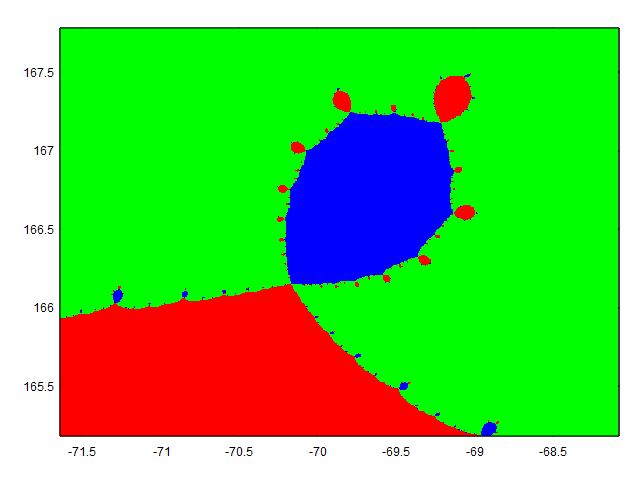
\includegraphics[width=0.5\textwidth]{mandel_zoom2.png}
    \newline
\hspace{-6em}Fractal dibuxat pel polinomi $p(z)=(z-1.7693)(z-0.88465-0.58983i) (z+0.88465-0.58983i) $
\label{fig:prodcte arrels}
\end{center}
\newpage

\begin{center}
    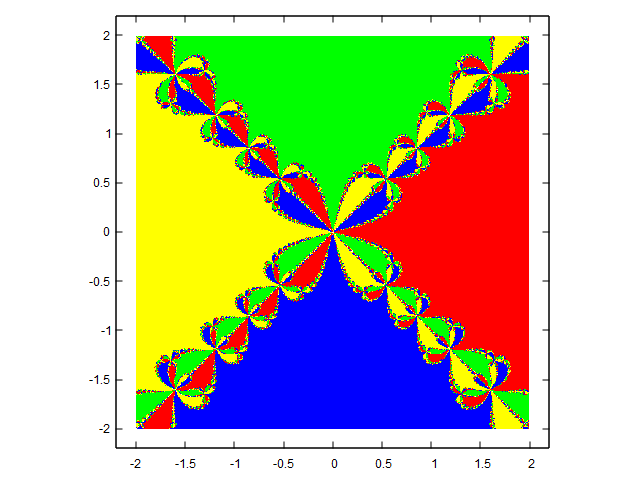
\includegraphics[width=0.6\textwidth]{z4_noZ.png}
    \newline
    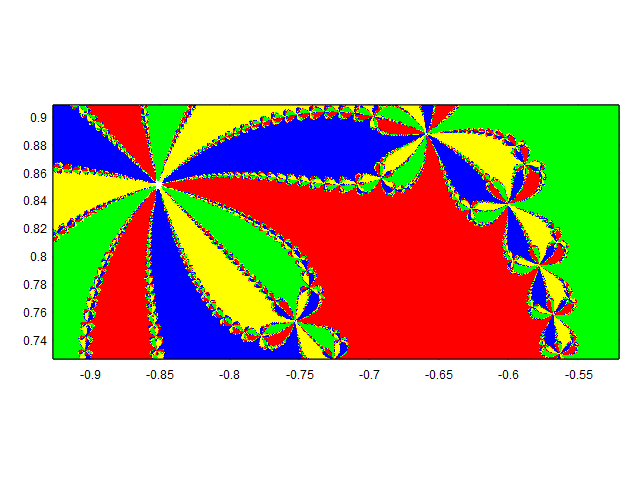
\includegraphics[width=0.6\textwidth]{z4.png}
    \newline
    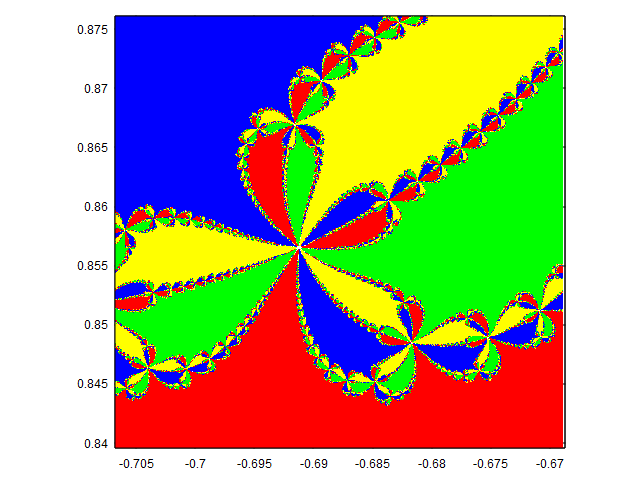
\includegraphics[width=0.5\textwidth]{z4_zoom2.png}
    \newline
\hspace{-6em}Fractal dibuxat pel polinomi $p(z)=z^4-1$
\label{fig:prodcte arrels}
\end{center}
\newpage

\begin{center}
    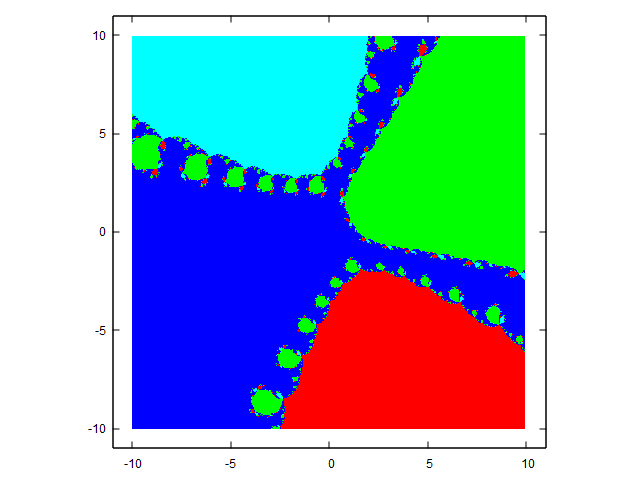
\includegraphics[width=0.6\textwidth]{z4R.png}
    \newline
    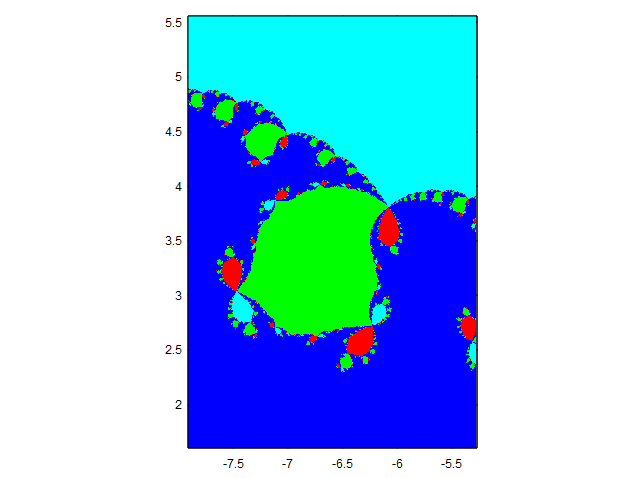
\includegraphics[width=0.6\textwidth]{z4R_zoom.png}
    \newline
    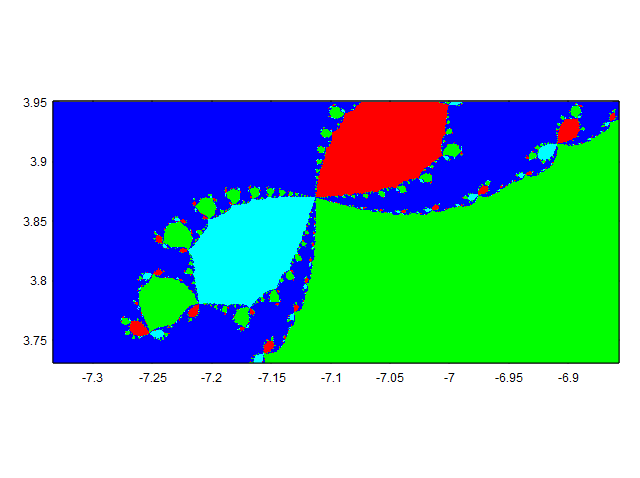
\includegraphics[width=0.5\textwidth]{z4R_zoom2.png}
    \newline
\hspace{-6em}Fractal dibuxat pel polinomi $p(z)=z(z-2+3i)(z+1-4i)(z-2-i) $
\label{fig:prodcte arrels}
\end{center}
\newpage

\begin{center}
    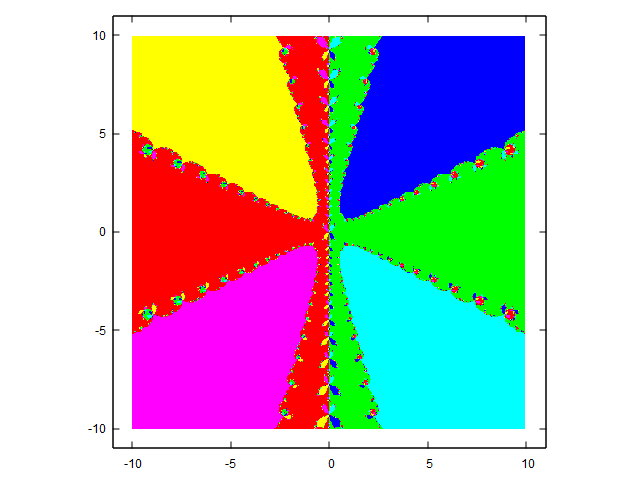
\includegraphics[width=0.6\textwidth]{z6.png}
    \newline
    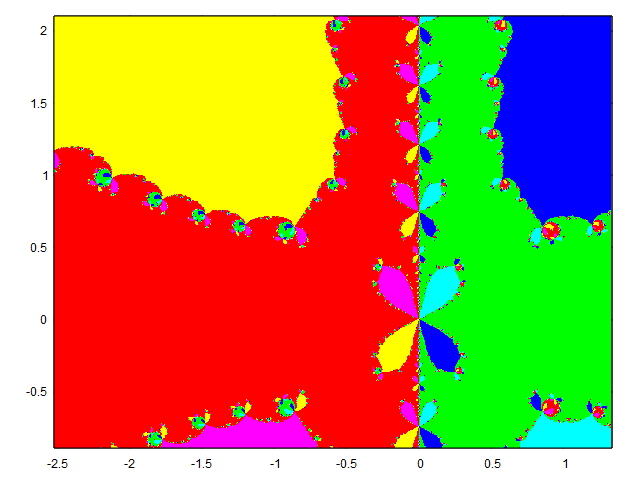
\includegraphics[width=0.6\textwidth]{z6_zoom.png}
    \newline
    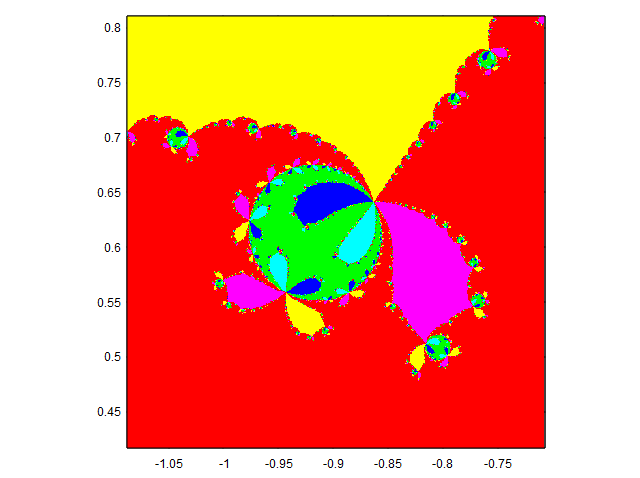
\includegraphics[width=0.5\textwidth]{z6_zoom2.png}
    \newline
\hspace{-6em}Fractal dibuxat pel polinomi $p(z)=(z+1)(z+1+i)(z+1-i)(z-1)(z-1+i)(z-1-i) $
\label{fig:prodcte arrels}
\end{center}
\newpage

\begin{center}
    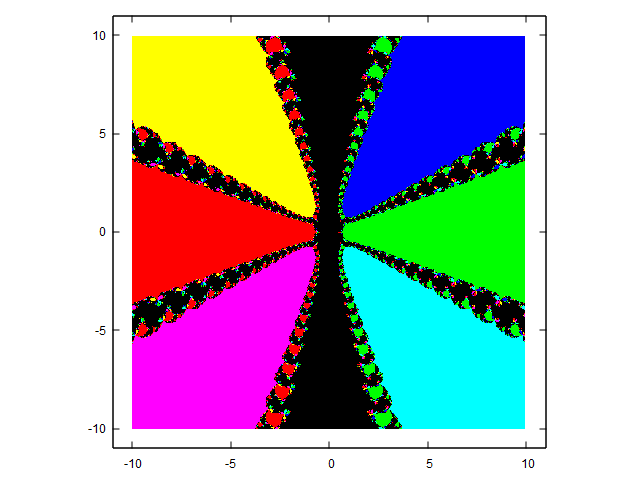
\includegraphics[width=0.6\textwidth]{z7.png}
    \newline
    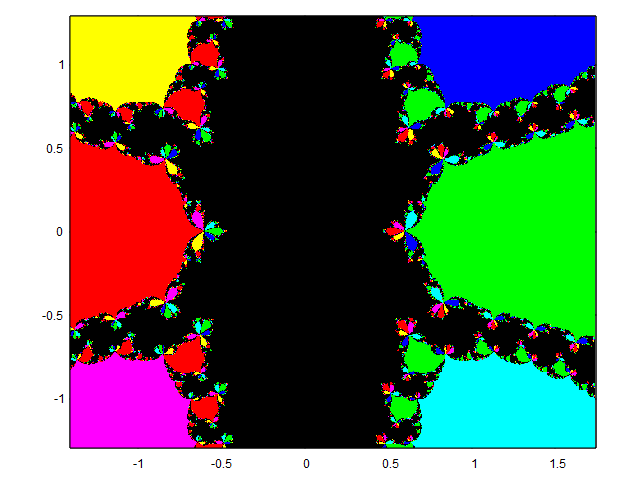
\includegraphics[width=0.6\textwidth]{z7_zoom.png}
    \newline
    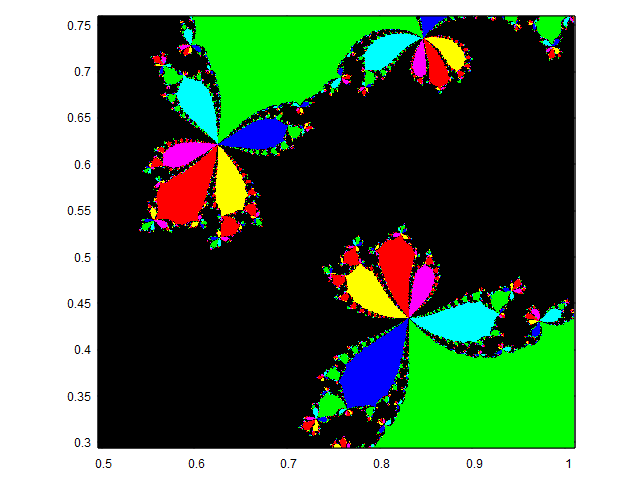
\includegraphics[width=0.5\textwidth]{z7_zoom2.png}
    \newline
\hspace{-6em}Fractal dibuxat pel polinomi $p(z)=z(z+1)(z+1+i)(z+1-i)(z-1)(z-1+i)(z-1-i) $
\label{fig:prodcte arrels}
\end{center}
\newpage


$$\sum_{k=0}^{\infty} e^{-\lambda} \cdot \lambda^{2K} / (2k)! = e^{-\lambda} \cdot (1/2) \cdot (e^{\lambda} + e^{-\lambda}) = (1+e^{-2 \cdot
\lambda})/2$$

\end{document}

